
\documentclass[12pt]{article}
\usepackage[russian,english]{babel}
\usepackage[backend=biber,style=numeric,sorting=none]{biblatex}
\usepackage{csquotes}
\addbibresource{sources.bib} %% подключение библиографической базы из файла sample.bib
\usepackage{fontspec}
\usepackage{listings}
\usepackage{url}
\usepackage[unicode, pdftex]{hyperref}
\usepackage[dvips]{graphicx} %вставка графики
\graphicspath{{images/}}%путь к рисункам
 \usepackage[a4paper,top=2cm,bottom=2cm,left=3cm,right=3cm,marginparwidth=1.75cm]{geometry}
\usepackage{ctable}
\setmainfont{Times New Roman}
\usepackage{amsmath}

\bibliography{sources.bib}

\lstdefinestyle{C}{               
    numbers=left,
    numbersep=10pt,
    breaklines=true
}

\begin{document}
\begin{titlepage}
\begin{figure}
    \begin{center}
        
\includegraphics[width=0.06\textwidth]{img/znachok_dvfu.png}
    \end{center}
\end{figure}
\thispagestyle{empty}

\begin{small}

\renewcommand{\baselinestretch}{2.0} % Полуторный интервал
\centerline{\large{МИНИСТЕРСТВО НАУКИ И ВЫСШЕГО ОБРАЗОВАНИЯ РОССИЙСКОЙ}}
\centerline{\large{ФЕДЕРАЦИИ}}
\centerline{Федеральное государственное автономное образовательное учреждение}
\centerline{высшего образования}
\centerline{\textbf{«Дальневосточный федеральный университет»}}
\centerline{\textbf{(ДВФУ)}}

\noindent\rule{\textwidth}{4pt}
\specialrule{.1em}{.05em}{.05em}

\centerline{\textbf{ИНСТИТУТ МАТЕМАТИКИ И КОМПЬЮТЕРНЫХ ТЕХНОЛОГИЙ}}
\centerline{\textbf{Департамент математического и компьютерного моделирования}}

\vfill

\vfill

\centerline{\textbf{Реферат}}
\centerline{\textbf{о практическом задание по дисциплине АИСД}}
\centerline{«Алгоритм поиска D*Lite»}
\par\noindent\rule{\textwidth}{0.3pt}
\centerline{направление подготовки 09.03.03 «Прикладная информатика»}
\centerline{профиль «Прикладная информатика в компьютерном дизайне»}

\vfill

\vfill

\noindent
\begin{tabular}{p{0.56\textwidth} p{0.70\textwidth}}
 & Выполнил студент  \\
 &  гр. Б9121-09.03.03пикд \\
 & Масличенко Елизавета Андреевна  \\
 & \parindent0pt \\
\end{tabular}

\vfill
\noindent
\begin{tabular}{p{0.56\textwidth} p{0.70\textwidth}}
 Доклад защищен:& Руководитель практики  \\
 С оценкой \hrulefill & Доцент ИМКТ А.С Кленин  \\
 
\end{tabular}

\noindent


\vfill

\centerline{г. Владивосток}
\centerline{2023}
\clearpage
\end{small}
\end{titlepage}
\newpage
\begin{center}
\section*{Оглавление}
\end{center}
    \hyperlink{a1}{\section{Введение}}
\hyperlink{a2}{\section{Авторы и история}}
\hyperlink{a3}{\section{Описание алгоритма и реализация}}
\hyperlink{b1}{\subsection{Постановка задачи}}
\hyperlink{b2}{\subsection{Концепция предшественников и приемников}}
\hyperlink{b3}{\subsection{Переформулировка: Сведите к минимуму повторные вычисления}}
\hyperlink{b4}{\subsection{Общий D* Lite:}}
\hyperlink{b5}{\subsection{Обработка изменения веса локально}}
\hyperlink{b6}{\subsection{Локальные несоответствия}}
\hyperlink{b7}{\subsection{Обновление и расширение узлов}}
\hyperlink{b8}{\subsection{Сверхсогласованный узел}}
\hyperlink{b9}{\subsection{Недостаточно согласованный узел}}
\hyperlink{b0}{\subsection{Перенос приоритетной очереди и изменение эвристики}}
\hyperlink{c1}{\subsection{Общий D* Lite(конкретизация):}}
\hyperlink{a4}{\section{Пример работы алгоритма}}
\hyperlink{a5}{\section{Тестирование и анализ производительности}}
\hyperlink{a6}{\section{Список литературы}}
\begin{center}
   \hypertarget{a1}{\section*{Введение}}
\end{center}
Мы собираемся использовать робота,находящегося в мире сетки.Он расположен в начальной точке,пытаясь добраться до цели.Он может двигаться вверх,вниз,вправо или по диагонали.Он может видеть только восемь ячеек вокруг себя,когда движеться через этот мир сетки.Мы даем довольно хорошую карту мира.Это карта,на которой есть мир до того,как он начнет двигаться.Могут появляться новые препятсвия или препятсвия могут исчезнуть.Идея состоит в том что он будет делать наблюдения по мере продвижения в этом мире и обновлять свой план,чтобы добраться до цели,основываясь на том,что он видит по мере движения. На рис.1 показана исходная карта,которую мы дали роботу. На рис.2 показан запланированый путь к достижению цели.
\begin{center}
        \includegraphics[width=0.3\textwidth]{img/motiv1.png}
        \caption{рис.1}
        \includegraphics[width=0.3\textwidth]{img/motiv2.png}
        \caption{рис.2}
\end{center}
Робот переместиться в следующую позицию,а затем поймет,что на пути который он планировал ранее,есть препятсвие и теперь он должен перепланировать что бы найти правильный путь к цели.Он перепланирует и продолжает двигаться по новому плану и теперь он находит еще одно препятсвие,которое должен обойти и делает то же самое(перепланирует).
\begin{center}
        \includegraphics[width=0.3\textwidth]{img/motiv3.png}
        \includegraphics[width=0.3\textwidth]{img/motiv4.png}
        \includegraphics[width=0.3\textwidth]{img/motiv5.png}
        \includegraphics[width=0.3\textwidth]{img/motiv6.png}
        \includegraphics[width=0.3\textwidth]{img/motiv7.png}
        \includegraphics[width=0.3\textwidth]{img/motiv8.png}
        \includegraphics[width=0.3\textwidth]{img/motiv9.png}
        \includegraphics[width=0.3\textwidth]{img/motiv10.png}
\end{center}
Он продолжает проходить пока не доходит до точки,где мы имеем изменение в окружающей среде.Изменение представленно тем,что эти две клетки становяться черными и прошлый план становиться недействительным.Мы хотим, чтобы робот снова перепланировал,чтобы найти новый и оптимальный путь к цели.
\begin{center}
        \includegraphics[width=0.6\textwidth]{img/envairoment1.png}
        
\end{center}
\begin{center}
        \includegraphics[width=0.3\textwidth]{img/envairoment2.png}
        \includegraphics[width=0.3\textwidth]{img/envairoment3.png}
        \includegraphics[width=0.3\textwidth]{img/envairoment4.png}
        \includegraphics[width=0.3\textwidth]{img/envairoment5.png}
        \includegraphics[width=0.3\textwidth]{img/envairoment6.png}
        \includegraphics[width=0.3\textwidth]{img/envairoment7.png}
        \includegraphics[width=0.3\textwidth]{img/envairoment8.png}
        \includegraphics[width=0.3\textwidth]{img/envairoment9.png}
        \includegraphics[width=0.3\textwidth]{img/envairoment10.png}
        \includegraphics[width=0.3\textwidth]{img/envairoment11.png}
        \includegraphics[width=0.3\textwidth]{img/envairoment12.png}
        \includegraphics[width=0.3\textwidth]{img/envairoment13.png}     
\end{center}
\begin{center}
   \hypertarget{a2}{\section*{Авторы и история}}
\end{center}
\textbf{Алгоритм D star Lite} — алгоритм поиска кратчайшего пути во взвешенном ориентированном графе, где структура графа неизвестна заранее или постоянно подвергается изменению. Разработан Свеном Кёнигом и Максимом Лихачевым в 2002 году.\\
\textbf{Применение}\\
$D star$ и его варианты широко использовались для мобильной навигации роботов и автономных транспортных средств. Современные системы, как правило, основаны на $D star Lite$, а не на оригинальном $D star$ или сфокусированном $D star$. Фактически, даже лаборатория Стенца использует $D star Lite$, а не $D star$в некоторых реализациях. К таким навигационным системам относятся прототипная система, протестированная на марсоходах Opportunity и Spirit, и навигационная система победителя конкурса DARPA Urban Challenge, разработанные в Университете Карнеги-Меллона.
\begin{center}
   \hypertarget{a3}{\section*{Описание алгоритма и реализация}} 
\end{center}
\hypertarget{b1}{\subsection*{Постановка задачи}}
Задача заключается в том,чтобы эффективно добраться от цели до старта поэтапно планируя путь ,в изменяющимся пространстве.\\
$D star Lite$ - это алгоритм выполняющий поиск от одного начального узла к другому целевому(конечному,следующему узлу).По мере того как мы видим что на пути происходят изменения,мы будем это корректировать и учитывать.$D star Lite$-рассматривают с двух точек зрения.\\
Первая точка зрения должна думать как о модификации основного пространства.В своей первой итерации или при первом прогоне до каких-либо модификаций он ведет себя похоже на алгорит $A star$ а именно мы производим поиск от начального узла к узлу цели, мы сортируем узлы в очереди по общей стоимости, которая является суммой,значения g и h(эвристики)$f(s)=g(s)+h(s,s_{goal})$
\begin{itemize}
    \item $f(s)$ -общая стоимость узла(вершины)
    \item $g(s)$ - стоимость перехода от одно узла к другому
    \item $h(s,s_{goal})$ -эвристика стоимость получения узла от $s,s_{goal}$
\end{itemize}
Вторая точка зрения на алгорит $A star$ с точки зрения алгоритма Дейкстры,когда мы исправляем или изменяем граф,наши методы заключаются в том, что бы ослабить веса ребер пока они не достигнут своего истинного значения.Теперь, когда мы отличаемся от алгоритма Дейкстры используя $D star Lite$ мы выбираем только те узлы,которые хотим рационально(эффективно) использовать.В то время как алгоритма Дейкстры, пытаеться уместить(вычислить) весь граф.Мы хотим пройти только от одного начального узла к одному конечному узлу.\\
Теперь что обычно не рассматриваеться в алгоритме $A star$, но очень важно для $D star Lite$ так это то как различить два узла с одниковой общей стоимостью в очереде.\\
Итак мы вводим пару(introducing a couplet),состоящую из 2 значений $f(s)=<f_1(s),f_2(s)>$
\begin{itemize}
    \item $f_1(s)=g(s)+h(s,s_{goal})$Это линейная комбинация наших затрат на достижение конечного узла и эвристической функции.
    \item $f_2(s)=g(s)$ - стоимость перехода от одно узла к другому
    \item $f(s)=<g(s)+h(s,s_{goal}),g(s)>$
\end{itemize}
Таким образом порядок расширения узлов из очереди сначала упорядочивает их по значению $f1$  и если два узла имеют одинаковое значение $f1$, мы выбираем узел с наименьшим значение $g(s)$
\hypertarget{b2}{\subsection*{Концепция предшественников и приемников}}
Концепция предшественников(predecessor) и приемников(successors) любого заданного узла.В любом случае граф состоит из направленных ребер и у нас может быть граф с ненаправленными ребрами,но мы можем думать о любом ребре направленном  в обе стороны.\\
Концпепция \textbf{приемника} узла состоит в том что каждый узел может быть достигнут из данного узла по ребрам которые можно найти.\\
Концепция \textbf{предшественников} представлет собой каждый узел, из которого этот узел может быть достигнут, т.е. узлы от которых мы можем следовать по направленому ребру к узлу.
\begin{itemize}
    \item $Succ(s)$ -множество узлов(вершин) изсходящих из вершины $s$ .Таким образом приемниками($Succ(s)$) красного узла, являются вот эти два синих узла.
    \item \includegraphics[width=0.7\textwidth]{img/Succ(s).png}
    \item $Pred(s)$ - множество узло вершин входящих в вершину s.\\Таким образом предшественниками($Pred(s)$) красного узла, являются вот эти два синих узла.
    \item \includegraphics[width=0.7\textwidth]{img/Pred(s).png}
\end{itemize}
\hypertarget{b3}{\subsection*{Переформулировка: Сведите к минимуму повторные вычисления}}
Подумайте над $D star Lite$ в том смысле, что это повторяющийся поиск по принципу "лучше всего сначала"(best-first search).Когда принципы алгоритма $A star$ проявляються через граф с изменяющимися весами ребер по мере прохождения этого графа, что означает что по мере того как мы перемещаемся от нашего начального узла к нашему конечному узлу вдоль пути,который мы планируем мы можем видеть что веса ребер меняются.
\begin{center}
        \includegraphics[width=1.1\textwidth]{img/primer1.png}
\end{center}
И в этом примере я моделирую препятсвие возникающее между этим узлом и целью, что означает что мы удалили ребро.И это фактически то же самое что и изменение веса ребра.Моделируем это изменение веса до значения  бесконечности, что означает что по этому ребру нельзя двигаться.\\
Мы рассматриваем это как перепланирование за счет уменьшение стоимости пути.Как только мы переместились $ s_{start}$ как мы найдем путь отсюда к $ s_{goal}$,когда это ребро по сути удалено?
\begin{center}
        \includegraphics[width=1.1\textwidth]{img/primer2.png}
\end{center}
Поэтому мы хотим сделать $D star Lite$ эффективным.И это повторный поиск по графу по мере его обхода. Поскольку мы используем эти значения $g(s)$ и если мы сохраним формулировку того, что мы измеряем растояние, которое нужно пройти или достичь узла от нашего начального узла.Эта формулировка не сохраняеться, когда мы перемещаем наш $ s_{start}$. Перемещение начально узла происходит при обновлении позии робота. \\
\\
Перейдем к примеру.Значение $g_1(s)$ или стоимость перехода от одного начального узла к другому  представляет комбинацию 2 ребер на примеер Case1:таким образом $g_1(s)=2+2=4$\\Теперь когда мы движемся по тому пути,который мы спланировали к следующему узлу прошлое значение $g_1(s)\neq g_2(s)$ не сохранилось  на примере Case2.
\begin{center}
        \includegraphics[width=1.1\textwidth]{img/primer3.png}
\end{center}
Так что мы делаем это переформулируем наш поиск,чтобы начать \textbf{искать в противоположном направлении}.Теперь мы измеряем для наших значений g стоимость достижения цели от конкретного узла. И вместо эвристики измеряем затраты, чтобы добраться от конкретного узла или добраться от начального к конкретному.И так ищем от цели $ s_{goal}$ назад по графу. \\
В этом случае независимо от того,являеться ли узел начальным,мы сохраняем значение $g(s)$ и стоимость путешствия от текущего узла к цели.Мы сохраним эту формулировку для максимальной эффекивности.
\hypertarget{b4}{\subsection*{Общий D* Lite:}}
\begin{enumerate}
    \item Инициализируйте все узлы как нерасширенные.
    \item Выполнить поиск по принципу "best-first search"(лучший — первый)от конечного узла к начальному, пока начальный узел не согласуеться со своими соседями
    \item Затем мы перемещаем начальный узел в следующую лучшую вершину(по созданному ранее нами плану)
    \item Если какие-либо граничные затраты изменились(имееть ввиду стоимость ребер):
    \begin{enumerate} 
        \item отследить как изменилась эвристика
        \item обновить исходные узлы измененных ребер
    \end{enumerate}
    \item Повторить пункт №2
\end{enumerate}
\hypertarget{b5}{\subsection*{Обработка изменения веса локально}}
Как мы справляемся с изменением веса локально на месте.И делаем это потому что не хотим отслеживать изменение веса на протяжении всего графика.Мы хотим справиться с эти эффективно,поэтому нам нужно обрабатывать только те изменения,которые действительно влияют на нашу проблему.\\
Пример заключаеться в том,что я изменила стоимость веса ребра с 6 на 1.И теперь мы можем добраться до красного узал по новому оптимальному пути.Новое значение $g(s)=5$.Но это не сохранилось.
\begin{center}
        \includegraphics[width=1.1\textwidth]{img/primer4.png}
\end{center}
\begin{center}
        \includegraphics[width=0.6\textwidth]{img/primer5.png}
\end{center}
Затем эти изменения распространяються на наших предшественников $Pred(s)$, потому что стоимость каждого процесса зависит от значения $g(s)$ для их приемника.И поэтому когда мы попадаем в узел, мы должны распространить это изменение по всему граффу.Поэтому,что бы сделать это эффективно мы используем подход подобный $A star$,где мы сначала обновляем узлы с наименьшей стоимостью и мы не расширяем узел,пока он не станет следующим с наименьшей стоимостью.
\begin{center}
        \includegraphics[width=1\textwidth]{img/primer6.png}
\end{center}
Что бы решить проблему, мы собираемся хранить дополнительное значение 
\begin{center}
       $rhs(s)=min_{s'\in Succ(s)}(g(s')+с(s,s')$
\end{center}

(англ. right-hand side value) И когда ваше значение $rhs(s)\neq g(s)$ это называеться,то что имеем как \textbf{локальная несогласованность.}
Учитывая логику значение $rhs(s)$ должно быть таким,каким будет скоректированно ваше значение $g(s)$.Таким образом при изменении стоимости ребра $rhs(s)=4+1=5$
\hypertarget{b6}{\subsection*{Локальные несоответствия}}
У нас есть 2 типа локального несоотвествия
\begin{itemize}
    \item $g(s)>rhs(s)$ локально сверхосласованно
    \item $g(s)<rhs(s)$ локально недостаточно согласованно
\end{itemize}
\hypertarget{b7}{\subsection*{Обновление и расширение узлов}}
\begin{center}
        \includegraphics[width=0.5\textwidth]{img/primer7.png}
        \caption{рис.1}
        \includegraphics[width=0.5\textwidth]{img/primer8.png}
        \caption{рис.2}
\end{center}

Под "обновлением узлов" я подразумеваю повторное вычисление значения $rhs(s)$ а затем помещение этого узла в очередь приоритетов,если этот узел локально несовместим.Что бы привести пример я изменила значение стоимость ребра с 6 на 1 предварительно подсчитав на рисунке 1 значение $rhs(s)=7$ до изменений и на рисунке 2 после изменений $rhs(s)=5$.Теперь мы видим на рис.2, что узел локально несогласован.\\
И поэтому мы помещаем его в очередь приоритетов.рис.3
\begin{center}
        \includegraphics[width=0.7\textwidth]{img/primer9.png}
        \caption{рис.3}
\end{center}
Значение приоритетной очереди основанно на этой формуле\\
$Q = <min[g(s),rhs(s)]+h(s,s_{start}),min[g(s),rhs(s)]>$\\
Оно основано на том как мы види значение $g(s)$ $rhs(s)$.Мы хотим взять минимальное значение одногого из них,что бы мы могли обрабатывать его в первый раз,когда оно вызовет изменения,распространяющиеся по графу.Таким образом это наш порядок в приоритетной очереди.
\begin{center}
        \includegraphics[width=0.7\textwidth]{img/primer10.png}
        \caption{рис.4}
\end{center}
Итак мы расширяем наши предыдущие узлы удаляя из очереди приоритетов и изменяя значение $g(s)$.Значения $g(s)$ уменьшаються до значения $rhs(s)$,поэтому мы просто устанавливаем $g(s)=rhs(s)$.В этом случае узел локально непротеричив(согласован) и он остается таким.
\begin{center}
        \includegraphics[width=0.7\textwidth]{img/primer11.png}
        \caption{рис.5}
\end{center}
Почему происходит процесс изменения $rhs(s)$ и отслеживаю это новое значение для того,что бы поставить в очередь,а затем снова убрать его,вместо того чтобы просто пересчитать значение $g(s)$ ? Можно подумать что вы добавляете что-то в очередь,если мы незамедлительно обновим $g(s)$,существует несколько узлов,которые могут изменить один и тот же узел,который мы только-что рассмотрели.Под этим я подразумеваю дополнительные изменения работы по мере их распространения обратно по графу,которые могут привести к изменению значения правой стороны это конкретного узла.Что нам нужно сделать если мы можем пересчитывать g(s) каждый раз так это поставить его в очередь,сигнализируя о том что мы пересчитываем g(s) и выполнить этот перерасчет, а затем новые изменения которые мы сделали делая это снова и снова и снова и мы хотим избежать этой ситуации.\\
Мы хотим сохранить $rhs(s)$ как временное значение.Которое можно изменить,когда оно находиться в очереде.Итак,когда что-то стоит в очереди, оно есть там один раз и его можно обновить и снять.Но мы знаем когда его сняли,что он был снят в нужно время и его не нужно будет снова обрабатывать.
\hypertarget{b8}{\subsection*{Сверхсогласованный узел}}
\begin{center}
          $g(s)>rhs(s)$
\end{center}
\begin{itemize}
    \item Стоимость нового пути $rhs(s)$ лучше, чем стоимость старого пути $g(s)$.
    \item Немедленно обновите $g(s)$ до $rhs(s)$ и распространите на всех предшественников
    \item Установить $g(s) = rhs(s)$
    \item Обновление всех предшественников узла $s$
\end{itemize}
Узел теперь локально согласован и он останется таким.
\hypertarget{b9}{\subsection*{Недостаточно согласованный узел}}
\begin{center}
          $g(s)<rhs(s)$
\end{center}
\begin{itemize}
    \item Стоимость старого пути $g(s)$ лучше, чем стоимость нового пути $rhs(s)$
    \item Задержите расширение вершины и распространитесь на все предшественники
    \item Установить $g(s) = \infty$
    \item Обновление всех предшественников узла $s$ и сам $s$
\end{itemize}
Вершина теперь локально согласована или локально сверхсогласованна. Она будет оставаться в
очереде до тех пор, пока $rhs(s)$ не станет следующей наилучшей стоимостью\\
Логика того,к какому типу относиться значение $rhs(s)$ реализована в функции $computeShortestPath()$
\begin{lstlisting}[language=C,style=C]
int Dstar::computeShortestPath() {

    list<state> s;
    list<state>::iterator i;

    if (openList.empty()) return 1;
    int k=0;
    while ((!openList.empty()) &&
           (openList.top() < (s_start = calculateKey(s_start))) ||
           (getRHS(s_start) != getG(s_start))) {

        if (k++ > maxSteps) {
            return -1;
        }
        state u;
        bool test = (getRHS(s_start) != getG(s_start));

        while(1) {
            if (openList.empty()) return 1;
            u = openList.top();
            openList.pop();
            if (!isValid(u)) continue;
            if (!(u < s_start) && (!test)) return 2;
            break;
        }
        ds_oh::iterator cur = openHash.find(u);
        openHash.erase(cur);
        state k_old = u;
        if (k_old < calculateKey(u)) { 
            insert(u);
        } else if (getG(u) > getRHS(u)) { 
            setG(u,getRHS(u));
            getPred(u,s);
            for (i=s.begin();i != s.end(); i++) {
                updateVertex(*i);
            }
        } else {   
            setG(u,INFINITY);
            getPred(u,s);
            for (i=s.begin();i != s.end(); i++) {
                updateVertex(*i);
            }
            updateVertex(u);
        }
    }
    return 0;
}
\end{lstlisting}
В строке 8 в цикле while происходит проверка локальной несогласованности узла.С 29 по 42 строчку проверка к какому типу относиться локально несогласованный узел.
\hypertarget{b0}{\subsection*{Перенос приоритетной очереди и изменение эвристики}}
Проблема в том что мы движемся $s_{start}$ к другому узлу. Наше эвристическое значение измеряеться от любого заданного узла до узла конечного.Поэтому когда наш начальный узел изменился эвристика не будет,такого же значения ,что и прежде как на новом узле.Итак мы хотим, то что уже находиться в очереди было сопастовимо с тем что мы вычисляется для нашего нового значения,что бы мы могли использовать нашу логику которые мы уже сделали.\\
Мы вводим что-то называемое ключевым модификатором.\\$k_m=k_m+h(s_{last},s_{start})$\\ Мы переходим от предыдущего начального узла,который здесь я указала как последний к новому начальному узлу.Тепер когда мы добавляем новые узлы в очередь,вместо того,чтобы вычитать это значение из всего что уже находиться в очереди,мы просто увеличиваем для всех узлов,которые мы помещаем в очередь,их значения на этот новый модификатор.Потому что когда мы выходим из очереди,все что имеет значение -это относительное различие между ними.Таким образом,вместо того,что бы вычитать значение из всего в очереди,добавление этого значения ко всем новым значениям,которые появляются в очереди,позволит достичь той же цели.\\
Формула приоритетной очереди изменяется:\\
$<min[g(s),rhs(s)]+h(s,s_{start})+k_m,min[g(s),rhs(s)]>$
\hypertarget{c1}{\subsection*{Общий D* Lite(конкретизация):}}
\begin{enumerate}
    \item Инициализация всех значений $g(s)=\infty$, $rhs(s,s_{goal})=\infty$, $rhs(s_{goal})=0$, $k_m=0$, $s_{last}=s_{start}$,
    \item Поиск по принципу"best-first search"(лучший — первый),пока$s_{start}$ не будет локально согласован и расширен
    \item Переместить $s_{start}=argmin_{s'\in Succ(s^{start})}(c(s_{start},s')+g(s'))$
     \item Если какие-либо стоимости ребер изменились
     \begin{enumerate} 
        \item $k_m=k_m+h(s_{last},s_{start})$
        \item Обновите $rhs(s)$ и положение в очереди для исходных узлов измененных ребер
    \end{enumerate}
    \item Повторите шаг № 2
\end{enumerate}
\begin{center}
   Всегда сортируйте по формуле:\\$<min[g(s),rhs(s)]+h(s,s_{start})+k_m,min[g(s),rhs(s)]>$\\
\end{center}


\begin{center}
   \hypertarget{a4}{\section*{Пример работы алгоритма}}
\end{center}
Рассмотрим краткий пример с пятью узлами.Робот начинает с узла А и его цель найти кратчайший путь к узлу G,за исключением того что граф может измениться по мере прохождением робота или робот может получить новую информацию.\\
Изначально робот думает что все узлы доступны.Он знает что все длины пути равны 1 за исключением пути от D до G=10.Это двунаправленный граф,каждое ребро идет в обоих направлениях.\\
Эвристика - это количество узлов до начального расстояния.
Все узлы правильно локально согласованны так как g(s)=rhs(s)\\

\begin{center}
        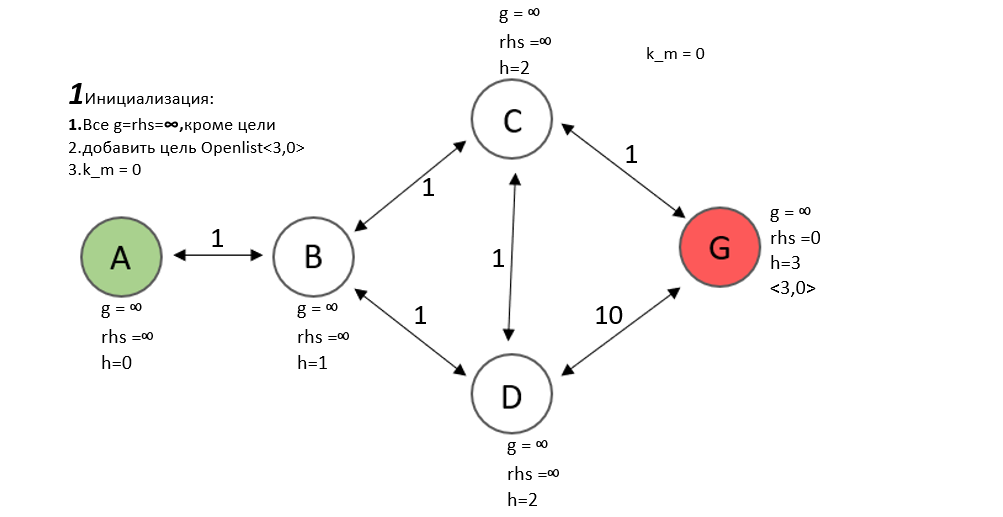
\includegraphics[width=1\textwidth]{img/example1.png}
    \end{center}
Мы помещаем вершину G в Openlist(очередь) используя формулу\\
$<min[g(s),rhs(s)]+h(s,s_{start})+k_m,min[g(s),rhs(s)]>$
Теперь у нас есть один узел(вершина в очереди).Так что нам придеться выйти из очереди.
\begin{itemize}
    \item удаляем узел G из OpenList
    \item проверка computeShortestPath(g(s)>rhs(s)),следовательно g(s)=rhs(s)=0
\end{itemize}
\begin{center}
        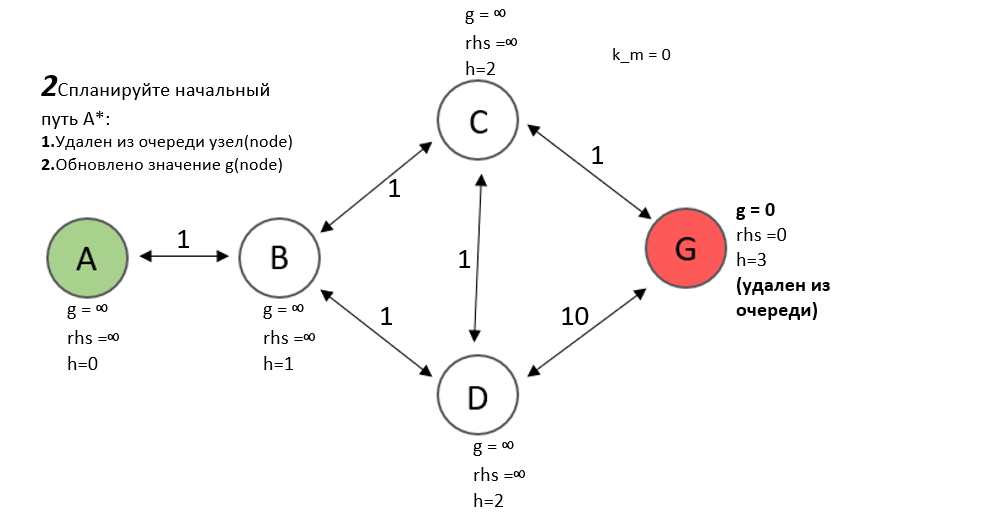
\includegraphics[width=1\textwidth]{img/example2.png}
    \end{center}    
Теперь мы собираемся обновить значения $rhs(s)$ соседей узла G  и в каждом случае значение будет минимальным по формуле $rhs(s)=min_{s'\in Succ(s)}(g(s')+с(s,s')$.И добавить в очередь $OpenList=[<3,2>;<12,10>]$
\begin{center}
        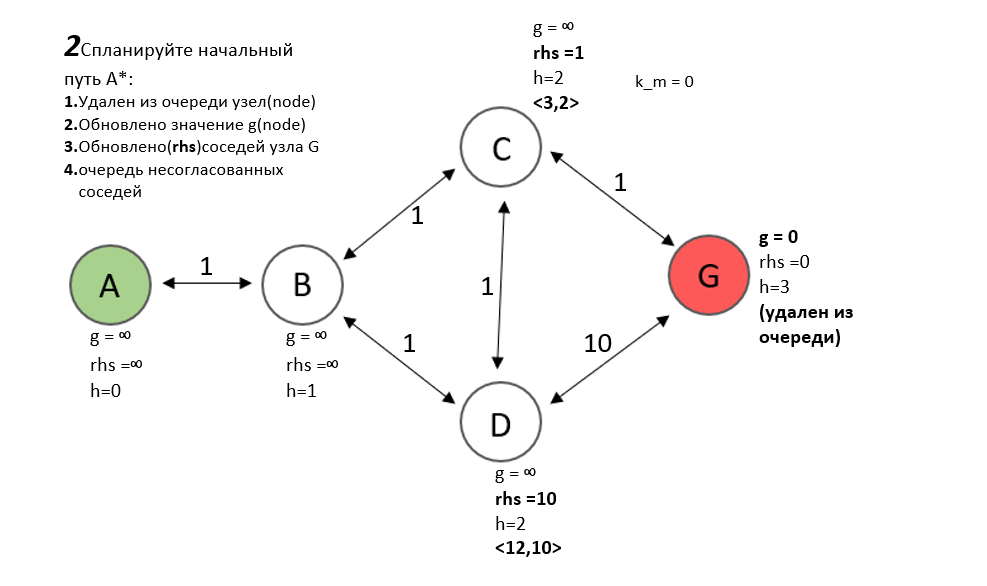
\includegraphics[width=1\textwidth]{img/example2_1.png}
    \end{center}
Теперь мы исключим из очереди еще один узел C так как у него наименьший ключ <3,1> .Проверка computeShortestPath(g(s)>rhs(s)),следовательно g(s)=rhs(s)=1 И обновим значения rhs(s) соседей узла C.\\Теперь в очереди $OpenList=[<3,2>;<4,2>]$
\begin{center}
        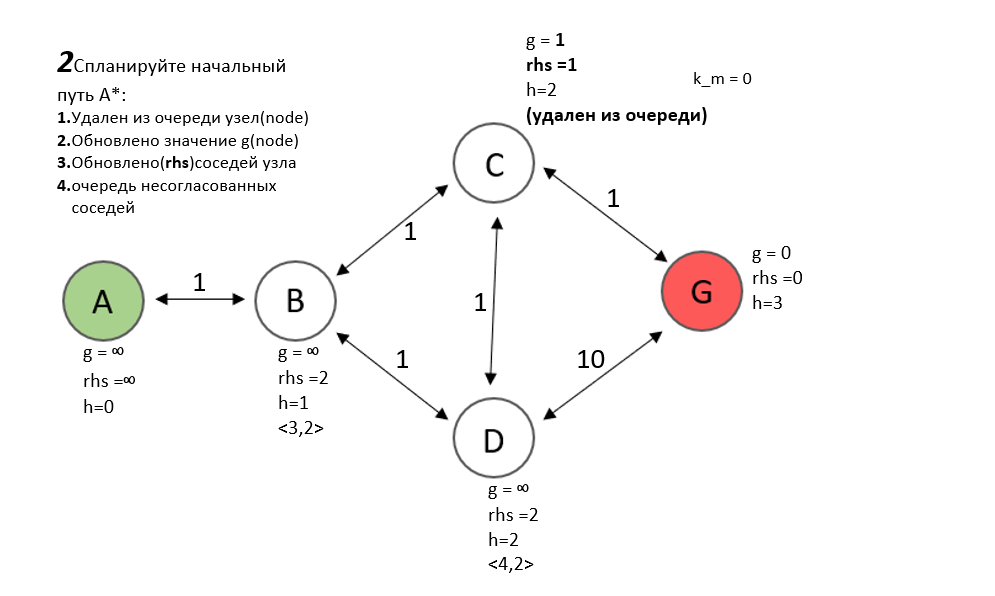
\includegraphics[width=1\textwidth]{img/example2_2.png}
    \end{center}
Дальше мы удаляем из очереди узел B так как у него наименьший ключ <3,2>Проверка computeShortestPath(g(s)>rhs(s)),следовательно g(s)=rhs(s)=2 И обновим значения rhs(s) соседей узла B.Мы не изменяем ключево значение узла D так как стоимость из G->C->D будет меньше чем из G->C->B->D
\\Теперь в очереди $OpenList=[<3,3>;<4,2>]$
\begin{center}
        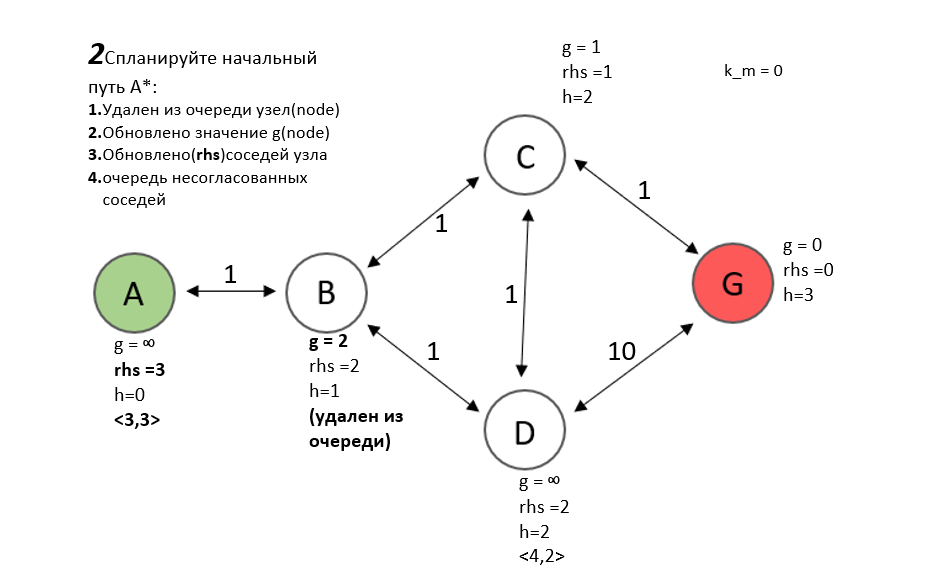
\includegraphics[width=1\textwidth]{img/example2_3.png}
    \end{center}
Далее мы удаляем из очереди узел A так как у него наименьший ключ.Проверка computeShortestPath(g(s)>rhs(s)),следовательно g(s)=rhs(s)=3. $OpenList=[<4,2>]$ И на это мы закончили.
\begin{center}
        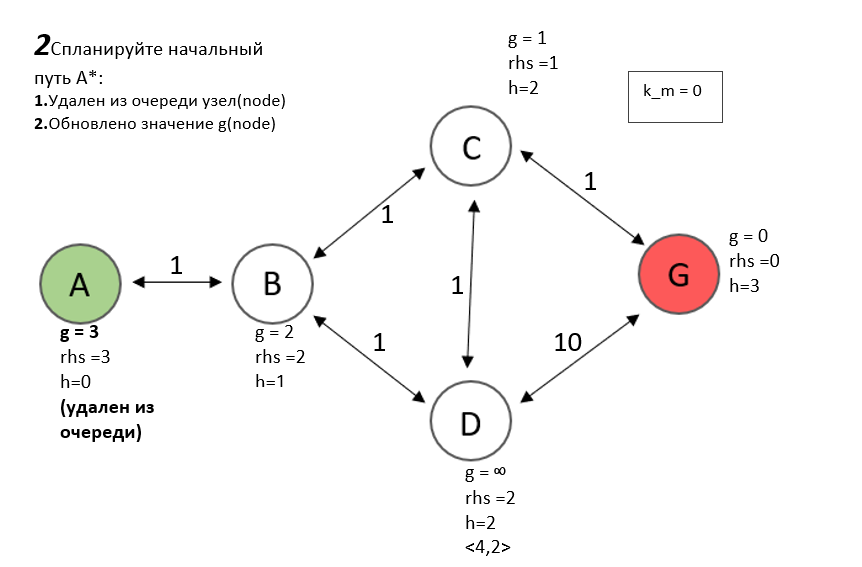
\includegraphics[width=1\textwidth]{img/example2_4.png}
    \end{center}
Робот переместился к своему следующему лучшему месту узлу B.Мы обновляем значения эвристики h для каждого узла в графе. Мы не изменяем очередь, но также должны обновить $k_m=1$ Появляеться препятсвие.В точке С есть препятсвие, которе робот теперь может видеть так как он ближе переместился к узлу C, но раньше он его не видел. Мы укажем эти изменения изменив ребра узла С на стоимость равной бесконечность.Это означает что робот никогда не сможет туда добраться.
\begin{center}
        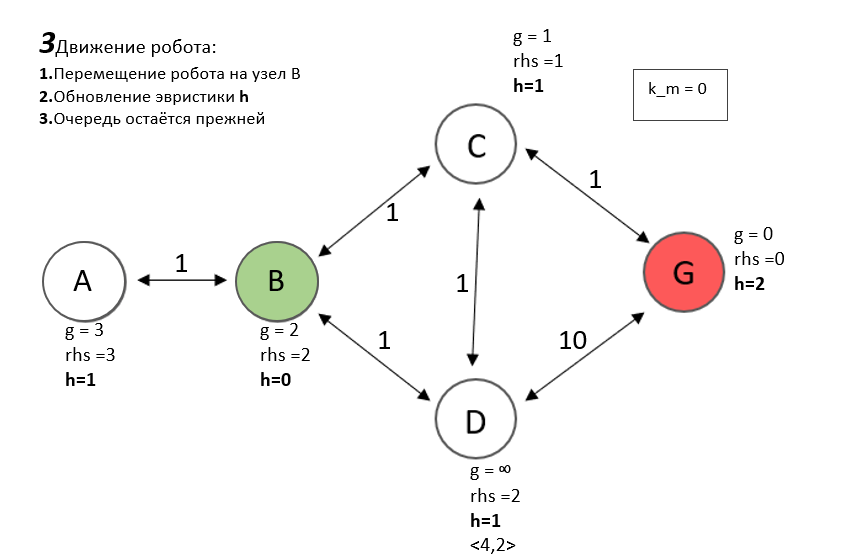
\includegraphics[width=1\textwidth]{img/example3.png}
         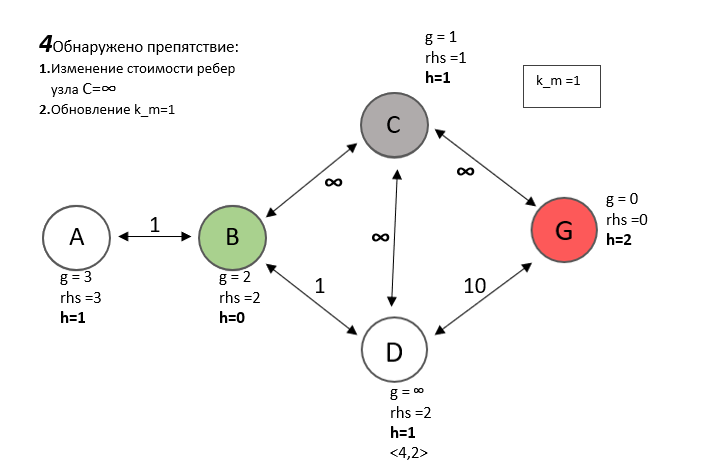
\includegraphics[width=1\textwidth]{img/example4.png}
    \end{center}
Далее мы собираемся обновить значения rhs узла B  и его соседей.\\$OpenList=[<3,1>;<3,2><5,3>]$
\begin{center}
         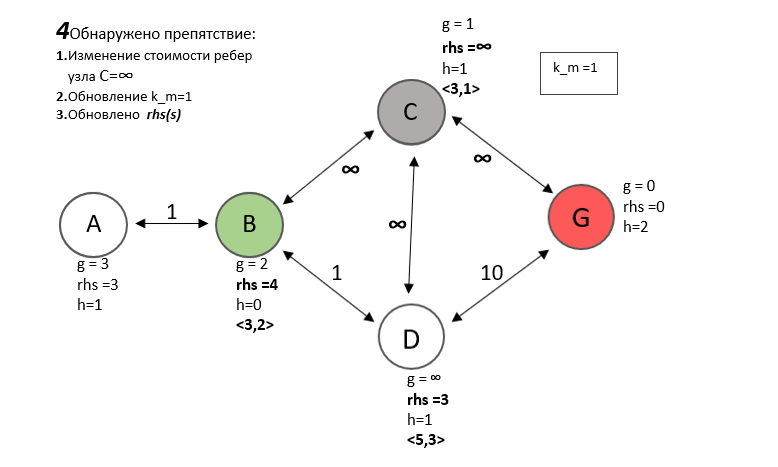
\includegraphics[width=1\textwidth]{img/example4_1.png}
    \end{center}
Далее мы удаляем из очереди узел C.Проверка $computeShortestPath(g(s)<rhs(s))$,следовательно $g(s)=\infty$
\begin{center}
         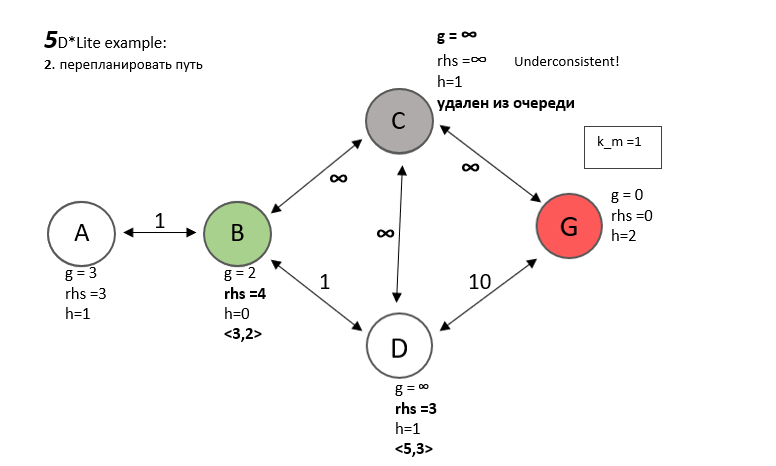
\includegraphics[width=1\textwidth]{img/example5.png}
    \end{center}
Далее мы удаляем из очереди узел B так как это наименьшее значение в очереди.Проверка 
$computeShortestPath(g(s)<rhs(s)) 2 < 4$,следовательно $g(s)=\infty$. Обновляем значение rhs  соседей и добавляем в OpenList изменившиеся значения.\\OpenList=[<5,3>;<12,10>]
\begin{center}
         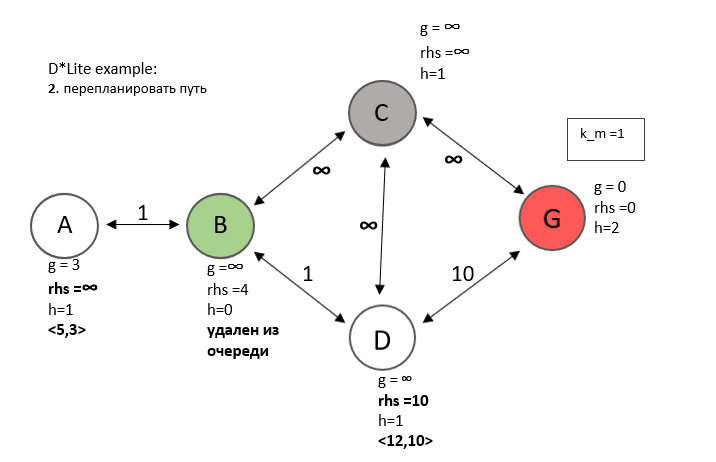
\includegraphics[width=1\textwidth]{img/example5_1.png}
    \end{center}
Так как <5,3> меньше чем <12,10> удаляем из очереди вершину А.\\Проверка 
$computeShortestPath(g(s)<rhs(s)) 3 < \infty $,следовательно $g(s)=\infty$. Обновляем значение rhs соседей и добавляем в OpenList изменившиеся значения.\\OpenList=[<12,10>;<12,11>]
\begin{center}
         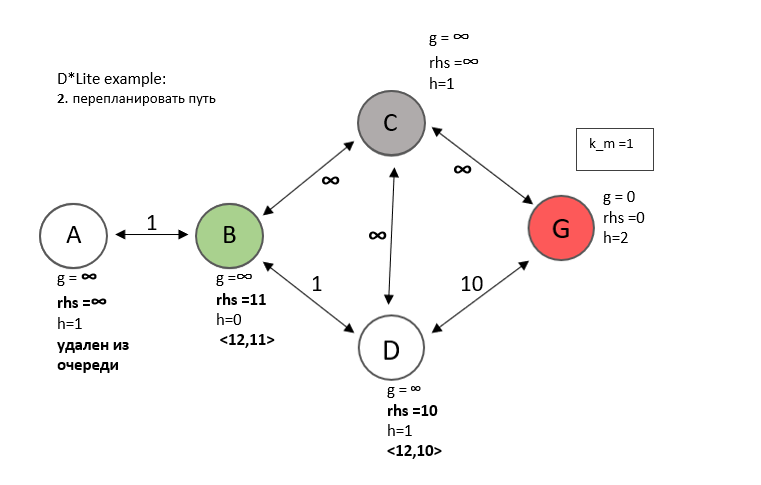
\includegraphics[width=1\textwidth]{img/example5_2.png}
    \end{center}
Так как <12,10> меньше чем <12,11> удаляем из очереди вершину D.\\Проверка 
$computeShortestPath(g(s)>rhs(s)) \infty >10 $,следовательно $g(s)=rhs(s)=10$. Обновляем значение rhs соседей и добавляем в OpenList изменившиеся значения.\\OpenList=[<12,11>]
\begin{center}
         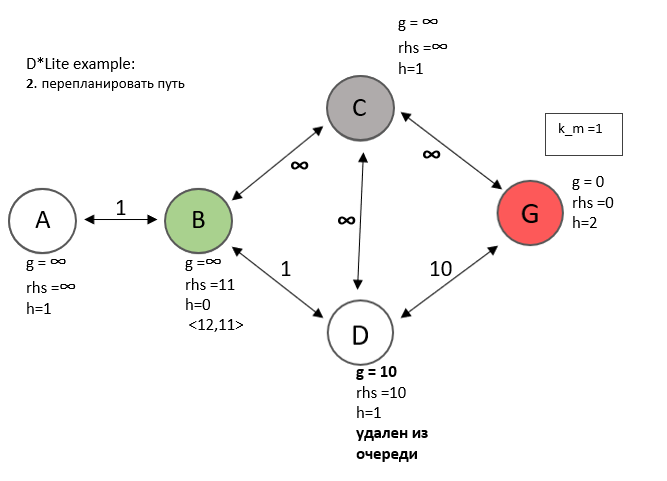
\includegraphics[width=1\textwidth]{img/example5_3.png}
    \end{center}
Удаляем из очереди вершину B.Проверка 
$computeShortestPath(g(s)>rhs(s)) \infty >11 $,следовательно $g(s)=rhs(s)=11$.Теперь узлы в графе локально согласованны. Обновляем значение rhs соседей и добавляем в OpenList изменившиеся значения.\\OpenList=[<14,12>] 
\begin{center}
         \includegraphics[width=1\textwidth]{img/example5_4.png}
    \end{center}
Мы нашли лучший и единственный путь из B->D->G  следовательно робот движеться в D.Изменяеться эвристика всех значений узлов на графе. Обновление значения $k_m=2$
\begin{center}
         \includegraphics[width=1\textwidth]{img/example6.png}
    \end{center}
Оказываеться препятсвие тоже движеться.Происходит изменение стоимости ребер узла вершины B,теперь их стоимость равна бесконечности.Также обнавляються значения rhs соседей вершины D.
В этом случае значение rhs(G) никогда не меняеться потому что растояние G до самой себя всегда будет равно нулю.
OpenList=[<4,1>,<14,1>]
\begin{center}
         \includegraphics[width=1\textwidth]{img/example6_1.png}
    \end{center}
Следовательно мы удаляем из очереди узел C.\\Проверка 
$computeShortestPath(g(s)>rhs(s)) \infty >1 $,следовательно $g(s)=rhs(s)=1$.\\Обновляем значение rhs соседей и добавляем в OpenList изменившиеся значения.\\OpenList=[<4,2>;<14,11>] 
\begin{center}
         \includegraphics[width=1\textwidth]{img/example6_2.png}
    \end{center}
Потом удаляем из очереди узел D.\\Проверка 
$computeShortestPath(g(s)>rhs(s)) 10 >2 $,следовательно $g(s)=rhs(s)=2$.\\Обновляем значение rhs соседей и добавляем в OpenList изменившиеся значения.\\OpenList=[<14,11>] 
\begin{center}
         \includegraphics[width=1\textwidth]{img/example6_3.png}
    \end{center}
Мы обнаружили путь из D->C->G и робот перемещаеться в узел C.Также обновляеться эвристика для всех улозлов графа.\\
Препятсвие не стоит на месте и приследует робота.Следовательно ребра узла D становяться стоять бесконечность. Также обновляться значение $k_m=3$ Обновляем значение rhs соседей и добавляем в OpenList изменившиеся значения.
\begin{center}
         \includegraphics[width=1\textwidth]{img/example7.png}
         \includegraphics[width=1\textwidth]{img/example7_1.png}
         \includegraphics[width=1\textwidth]{img/example8.png}
    \end{center}





    
\newpage  
\begin{center}
   \hypertarget{a5}{\section*{Тестирование и анализ производительности}}
\end{center}
Тесты написанны в формате in.txt out.txt в одной папке содержаться входные in.txt и выходняе данные out.txt.Всего 20 ручных тестов,позволяющих измерить время от количества размера данных.
\begin{center}
        \includegraphics[width=1.1\textwidth]{img/datetime.png}
    \end{center}
Также во все out.txt  я измеряю значение rhs(s) и g(s).На таблице представленно то как зависят функции от размера входящих данных.
\begin{center}
        \includegraphics[width=1\textwidth]{img/gtest.png}
    \end{center}
На данном графике произведен анализ состава $OpenList$(приоритеной очереди).А именно я сравниваю первое значение $k_{first}$ и $k_{second}$  взависимости от размера данных.
\begin{center}
        \includegraphics[width=1\textwidth]{img/openlisttest.png}
    \end{center}
\newpage  
\begin{center}
   \hypertarget{a6}{\section*{Список литературы}}
\end{center}

\nocite{*}
\printbibliography
\end{document}
